\documentclass[tikz,border=10pt]{standalone}
\usepackage{amsmath}
\usetikzlibrary{calc,shapes.geometric,arrows.meta,positioning}
\usepackage{xcolor}
\definecolor{accent}{HTML}{2D6BE4}
\definecolor{accentdark}{HTML}{1B4AA8}
\definecolor{codebg}{HTML}{F5F6F8}
\begin{document}
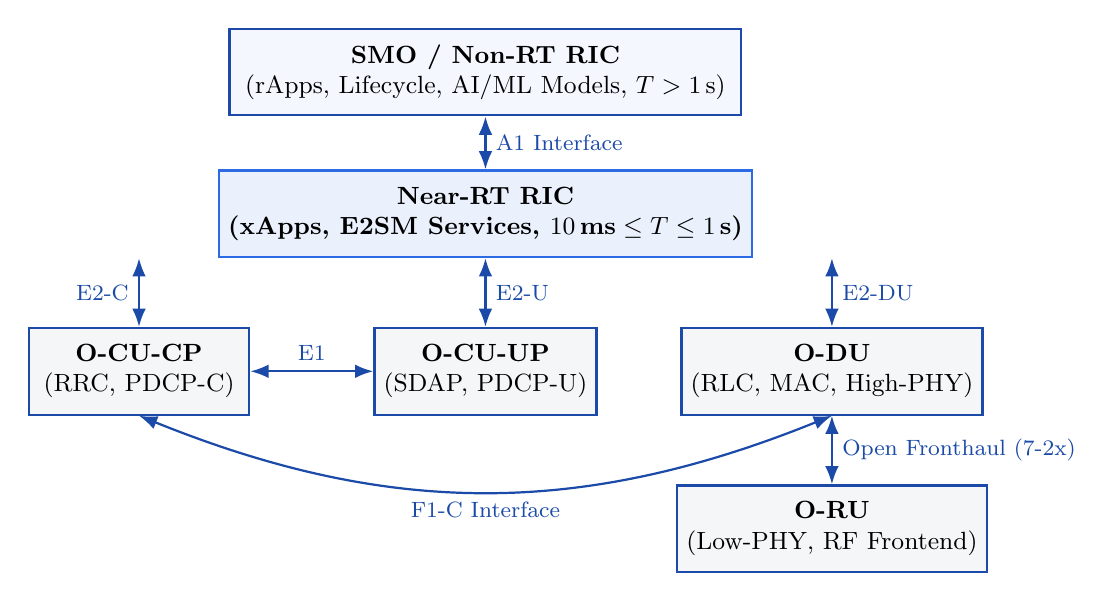
\begin{tikzpicture}[
    box/.style={rectangle, draw=accentdark, fill=codebg, thick, minimum width=2.8cm, minimum height=1.1cm, align=center, font=\small},
    ctrl/.style={rectangle, draw=accent, fill=accent!10, thick, minimum width=6.5cm, minimum height=1.1cm, align=center, font=\small\bfseries},
    arrow/.style={-Latex, thick, color=accentdark},
    darrow/.style={Latex-Latex, thick, color=accentdark}
  ]
  \node[box, fill=accent!5, minimum width=6.5cm] (smo) at (0, 3.8) {\textbf{SMO / Non-RT RIC}\\(rApps, Lifecycle, AI/ML Models, $T > 1$\,s)};
  \node[ctrl] (nearric) at (0, 2.0) {\textbf{Near-RT RIC}\\(xApps, E2SM Services, $10\,\text{ms} \le T \le 1\,\text{s}$)};
  
  \node[box] (cucp) at (-4.4, 0.0) {\textbf{O-CU-CP}\\(RRC, PDCP-C)};
  \node[box] (cuup) at (0, 0.0) {\textbf{O-CU-UP}\\(SDAP, PDCP-U)};
  \node[box] (du) at (4.4, 0.0) {\textbf{O-DU}\\(RLC, MAC, High-PHY)};
  \node[box, minimum width=3.4cm] (ru) at (4.4, -2.0) {\textbf{O-RU}\\(Low-PHY, RF Frontend)};

  \draw[darrow] (smo) -- node[right, font=\footnotesize] {A1 Interface} (nearric);
  \draw[darrow] (nearric.south -| cucp.north) -- node[left, font=\footnotesize] {E2-C} (cucp.north);
  \draw[darrow] (nearric.south) -- node[right, font=\footnotesize] {E2-U} (cuup.north);
  \draw[darrow] (nearric.south -| du.north) -- node[right, font=\footnotesize] {E2-DU} (du.north);
  \draw[darrow] (du) -- node[right, font=\footnotesize] {Open Fronthaul (7-2x)} (ru);
  \draw[darrow] (cucp) -- node[above, font=\footnotesize] {E1} (cuup);
  \draw[darrow] (cucp.south) to[bend right=22] node[below, font=\footnotesize] {F1-C Interface} (du.south);
\end{tikzpicture}
\end{document}
